% ============================================================
% ConsistXApp -- Part 1/3
% Target journal: Annals of Telecommunications
%
% IMPORTANT:
% 1. Use the official Springer Nature sn-jnl.cls.
% 2. Concatenate Parts 1, 2, and 3 in this order.
% 3. Replace every TODO before submission.
% 4. Do not reuse previous numerical results as results of the
%    revised algorithm without rerunning the experiments.
% ============================================================

\documentclass[pdflatex,sn-mathphys-num,iicol,oneside]{sn-jnl}

% \jyear{2026}

\usepackage{amsmath}
\usepackage{amssymb}
\usepackage{bm}
\usepackage{booktabs}
\usepackage{multirow}
\usepackage{array}
\usepackage{xcolor}
\usepackage{tikz}
\usepackage{url}
\usepackage{graphicx}

\usetikzlibrary{
    arrows.meta,
    positioning,
    fit,
    shapes.geometric
}

% ============================================================
% Macros
% ============================================================

\newcommand{\TODO}[1]{%
    \textcolor{red}{\textbf{[TODO: #1]}}%
}

\newcommand{\method}{\textsc{ConsistXApp}}
\newcommand{\legacy}{\textsc{VeriXApp}}
\newcommand{\gac}{\textsc{GAC}}
\newcommand{\cpsat}{\textsc{CP-SAT}}

\newcommand{\placeholderfigure}[2]{%
    \fbox{%
        \parbox[c][#2][c]{0.92\linewidth}{%
            \centering
            \textbf{Figure placeholder}\\[2mm]
            #1
        }%
    }%
}

\newtheorem{proposition}{Proposition}
\newtheorem{definition}{Definition}
\newtheorem{remark}{Remark}

\raggedbottom

\begin{document}

% ============================================================
% Title and authors
% ============================================================

\title[Consistency-Guided xApp Coordination]{
Consistency-Guided Finite-Domain xApp Coordination:
Incremental Propagation, Fractional-Stall Diagnosis,
and Explanation-Guided Exact Repair for O-RAN
}

\author*[1]{\fnm{Lillia} \sur{Ouali}}
\email{lillia.ouali@univ-bejaia.dz}

\author[2]{\fnm{Madani} \sur{Bezoui}}
\email{mbezoui@cesi.fr}

\author[1]{\fnm{Kamal} \sur{Amroun}}
\email{kamal.amroun@univ-bejaia.dz}

\author[3]{\fnm{Ahcene} \sur{Bounceur}}
\email{abounceur@sharjah.ac.ae}

\affil*[1]{
    \orgdiv{Department of Computer Science},
    \orgname{University of Bejaia},
    \orgaddress{
        \city{Bejaia},
        \country{Algeria}
    }
}

\affil[2]{
    \orgdiv{LINEACT},
    \orgname{CESI},
    \orgaddress{
        \city{Nancy},
        \country{France}
    }
}

\affil[3]{
    \orgname{University of Sharjah},
    \orgaddress{
        \city{Sharjah},
        \country{United Arab Emirates}
    }
}

% ============================================================
% Abstract
% ============================================================

\abstract{
The programmability of the Open Radio Access Network (O-RAN)
allows independently developed xApps to issue control requests
through the near-real-time RAN Intelligent Controller. Concurrent
requests may nevertheless be mutually incompatible, compete for
shared resources, or jointly violate service-level agreements.
We formulate multi-xApp arbitration as a dynamic finite-domain
constraint optimization problem in which action domains and
context-dependent conflict relations evolve between decision epochs.

We introduce \method, a consistency-guided coordination framework
combining incremental generalized arc consistency, continuous
relation-conditioned inference, fractional-stall diagnosis,
explanation-guided exact repair, and independent decision
verification. Generalized arc consistency soundly removes actions
that have no support in an incident hard relation before continuous
inference is executed. When propagation detects a domain wipeout,
its explanations identify a sufficient set of constraints and domain
restrictions responsible for the contradiction. When propagation
reaches a non-empty fixed point but continuous decoding remains
invalid, the same explanation mechanism guides the construction and
progressive expansion of an exact repair subproblem. Full-scope
constraint programming is retained as a deadline-bounded final
escalation, and no action is forwarded unless an independently
implemented verifier validates every registered hard constraint.

We prove that consistency filtering preserves all globally feasible
assignments while showing that generalized arc consistency alone
cannot eliminate symmetric fractional stalls. The evaluation compares
uncoordinated execution, static priorities, continuous-only
coordination, complete CP-SAT, GAC followed by CP-SAT, the original
radius-based repair strategy, and the proposed explanation-guided
framework on static and dynamic O-RAN conflict sequences.
We generated 15,000 unique decision epochs and evaluated ten methods on matched instances, yielding 150,000 method-epoch observations. In the separate static propagation suite, the pooled value- and tuple-reduction ratios are 21.7\% and 34.1\%, respectively.
It also reduces the
median exact-repair core size by 1.0 node, and attains
74.4\% feasibility and 56.8\% deadline compliance under strict 100ms bounds.
The study identifies the operating regimes in which
consistency-guided hybrid coordination is beneficial and those in
which complete CP-SAT remains preferable.
}

\keywords{
O-RAN,
xApp conflict management,
dynamic constraint satisfaction,
generalized arc consistency,
constraint propagation,
explanation-based repair,
fractional fixed points,
constraint programming
}

\maketitle

% ============================================================
\section{Introduction}
\label{sec:introduction}
% ============================================================

Open Radio Access Network (O-RAN) introduces disaggregation, open
interfaces, and programmable control into radio access networks.
A central component of this architecture is the RAN Intelligent
Controller (RIC), which supports applications operating at different
time scales. The non-real-time RIC hosts rApps, whereas the
near-real-time RIC hosts extended applications, referred to as xApps
\cite{polese2023oran}.

An xApp can implement a control function such as traffic steering,
mobility optimization, interference coordination, energy saving,
power control, or radio-resource allocation. Through the E2
interface, xApps receive network measurements and issue control
requests to E2 nodes. This programmability enables a multi-vendor
application ecosystem but also creates a coordination problem:
independently developed xApps may simultaneously attempt to control
the same parameter or pursue mutually incompatible performance
objectives.

The O-RAN Alliance identifies conflict mitigation between xApps as a
function of the near-real-time RIC \cite{oran2024conflict}. Existing
studies distinguish direct, indirect, and implicit conflicts
\cite{adamczyk2023conflict,wadud2024qacm}. Direct conflicts occur when
xApps request incompatible values for the same control parameter.
Indirect conflicts arise when different controlled parameters
influence a common key performance measurement (KPM). Implicit
conflicts occur when actions targeting distinct parameters or KPMs
interact through the dynamics of the radio access network.

Conflict management has been addressed through static priorities,
QoS-aware optimization, application profiling, digital twins,
game-theoretic mechanisms, and reinforcement learning
\cite{wadud2024qacm,prever2025pacifista,
giannopoulos2025comix,wadud2025mobility}. These approaches determine
or predict how candidate actions affect the network. A complementary
question arises after candidate actions and conflict relations have
been registered: how should a controller reason safely over finite
action domains under a strict control deadline?

This paper models xApp coordination as a dynamic finite-domain
constraint optimization problem. Each variable represents an accepted
xApp action, execution slot, target cell, power level, handover
configuration, or resource-allocation profile. Between two decision
epochs, active xApps, action domains, SLA thresholds, KPM dependencies,
and context-dependent conflict relations may change. Consecutive
coordination problems are therefore related rather than independent.

Two reasoning failures must be distinguished.

First, a candidate action may have no support in one or more incident
hard relations. Such a value can be removed soundly by constraint
propagation before continuous or exact optimization.

Second, every remaining value may possess local support while the
joint continuous state remains fractional. Deterministic decoding may
then combine individually supported values into an invalid assignment.
Generalized arc consistency is therefore useful but does not by itself
guarantee conflict-free decoding.

We introduce \method, a consistency-guided coordination framework
with five stages:

\begin{enumerate}
    \item dynamic finite-domain modelling of candidate xApp actions;
    \item incremental generalized arc-consistency propagation;
    \item continuous relation-conditioned inference on the filtered
    domains;
    \item fractional-stall diagnosis and explanation-guided exact
    repair;
    \item independent verification before an action is forwarded to
    the E2 interface.
\end{enumerate}

The propagation layer maintains explanations for value removals and
domain wipeouts. These explanations identify the constraints and
temporary decisions that contributed to a contradiction. They are
used to construct and progressively expand the exact repair core,
replacing a repair policy based only on a fixed radius in the conflict
graph.

The main contributions are as follows.

\begin{itemize}
    \item We formulate multi-xApp coordination as a dynamic
    finite-domain constraint optimization problem supporting direct,
    indirect, and implicit conflict relations.

    \item We introduce an incremental generalized arc-consistency
    layer that removes unsupported actions before continuous
    inference. The framework distinguishes restrictive updates from
    domain or relation relaxations, for which previously removed
    values may need to be restored.

    \item We prove that consistency filtering preserves all globally
    feasible assignments relative to the registered conflict model.

    \item We show that generalized arc consistency does not eliminate
    symmetric fractional stalls and therefore cannot replace joint
    decoding verification or exact repair.

    \item We define propagation explanations for explicit positive
    relations and use them to guide the construction and expansion
    of an exact repair subproblem.

    \item We distinguish propagation contradiction, operational
    fractional stall, invalid non-stalled decoding, local-repair
    infeasibility, and full-model infeasibility.

    \item We preserve an independently implemented decision verifier:
    no coordinated action is forwarded unless all registered hard
    relations are satisfied.

    \item We define an evaluation protocol covering domain reduction,
    propagation overhead, explanation quality, repair-core size,
    verified feasibility, deadline compliance, temporal stability,
    and network-level performance.
\end{itemize}

The remainder of this paper is organized as follows.
Section~\ref{sec:background} reviews O-RAN conflict management,
constraint propagation, and explanation-based repair.
Section~\ref{sec:model} presents the dynamic coordination model.
Section~\ref{sec:method} introduces \method.
Section~\ref{sec:analysis} establishes its propagation and
fractional-stall properties.
Section~\ref{sec:experiments} defines the experimental methodology.
Section~\ref{sec:results} reports the results.
Section~\ref{sec:limitations} discusses limitations and threats to
validity, and Section~\ref{sec:conclusion} concludes the paper.

% ============================================================
\section{Background and Related Work}
\label{sec:background}
% ============================================================

\subsection{O-RAN control architecture}

The O-RAN architecture includes the Service Management and
Orchestration framework, the non-real-time RIC, the near-real-time
RIC, and disaggregated RAN components such as the O-CU, O-DU, and
O-RU \cite{polese2023oran}.

The near-real-time RIC supports control loops typically operating
between tens of milliseconds and one second. xApps subscribe to
measurements, process network context, and issue E2 control requests.
Experimental frameworks such as ColO-RAN, OpenRAN Gym, and FlexRIC
facilitate the development and evaluation of programmable RAN
controllers
\cite{polese2022coloran,bonati2023openrangym,
schmidt2021flexric}. Recent work has also compared simulated,
emulated, hybrid, and hardware-based O-RAN experimentation platforms
under resource constraints \cite{navarro2026demystifying}.

Figure~\ref{fig:architecture} positions \method\ in the
near-real-time RIC control path. Candidate actions are propagated,
coordinated, repaired when required, and independently verified before
being forwarded through E2.

\begin{figure*}[t]
\centering
\resizebox{\textwidth}{!}{%
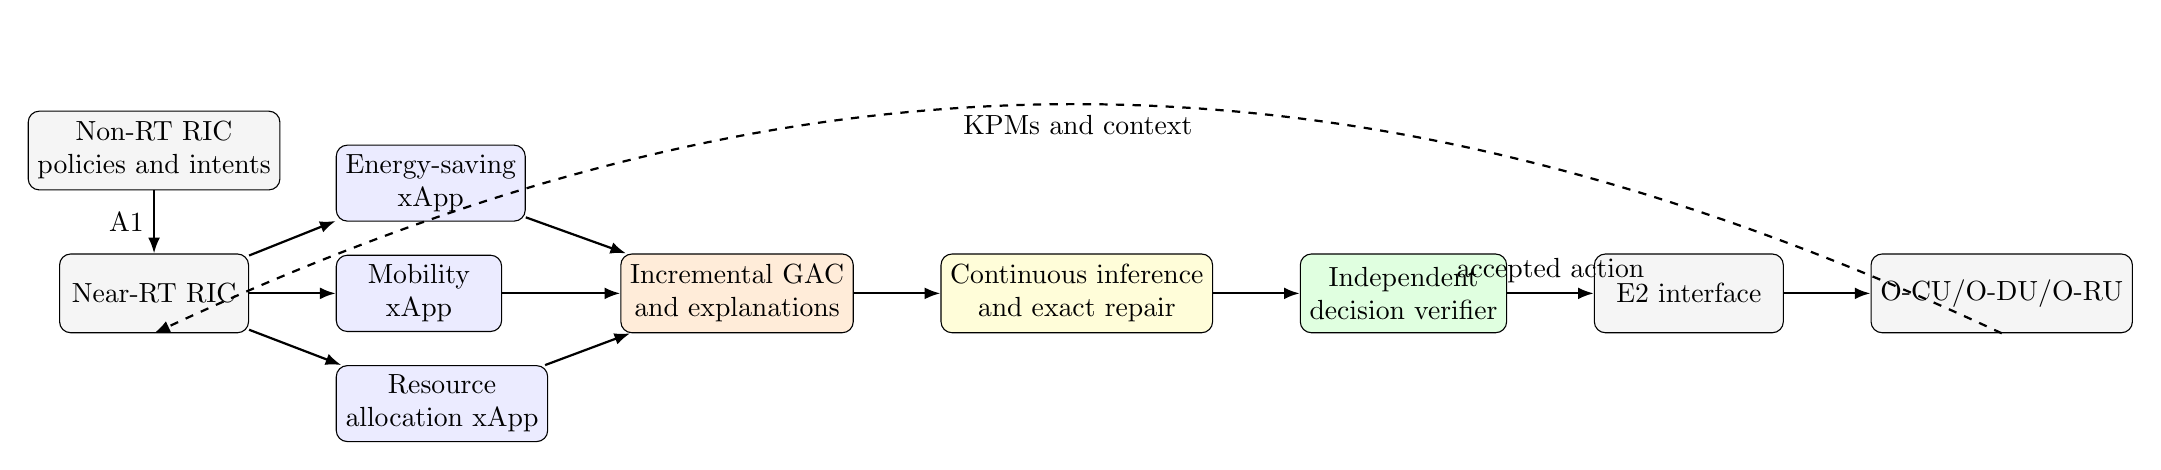
\begin{tikzpicture}[
    node distance=8mm and 11mm,
    block/.style={
        draw,
        rounded corners,
        align=center,
        minimum width=24mm,
        minimum height=10mm,
        fill=gray!8
    },
    app/.style={
        draw,
        rounded corners,
        align=center,
        minimum width=21mm,
        minimum height=9mm,
        fill=blue!8
    },
    prop/.style={
        draw,
        rounded corners,
        align=center,
        minimum width=26mm,
        minimum height=10mm,
        fill=orange!15
    },
    coord/.style={
        draw,
        rounded corners,
        align=center,
        minimum width=27mm,
        minimum height=10mm,
        fill=yellow!15
    },
    verify/.style={
        draw,
        rounded corners,
        align=center,
        minimum width=25mm,
        minimum height=10mm,
        fill=green!12
    },
    arrow/.style={-{Latex[length=2mm]},thick}
]

\node[block] (nonrt) {Non-RT RIC\\policies and intents};
\node[block, below=of nonrt] (near) {Near-RT RIC};

\node[app, right=of near, yshift=14mm] (x1)
{Energy-saving\\xApp};

\node[app, right=of near] (x2)
{Mobility\\xApp};

\node[app, right=of near, yshift=-14mm] (x3)
{Resource\\allocation xApp};

\node[prop, right=15mm of x2] (gac)
{Incremental GAC\\and explanations};

\node[coord, right=of gac] (coord)
{Continuous inference\\and exact repair};

\node[verify, right=of coord] (verifier)
{Independent\\decision verifier};

\node[block, right=of verifier] (e2)
{E2 interface};

\node[block, right=of e2] (ran)
{O-CU/O-DU/O-RU};

\draw[arrow] (nonrt) -- node[left]{A1} (near);

\draw[arrow] (near) -- (x1);
\draw[arrow] (near) -- (x2);
\draw[arrow] (near) -- (x3);

\draw[arrow] (x1) -- (gac);
\draw[arrow] (x2) -- (gac);
\draw[arrow] (x3) -- (gac);

\draw[arrow] (gac) -- (coord);
\draw[arrow] (coord) -- (verifier);
\draw[arrow] (verifier) -- node[above]{accepted action} (e2);
\draw[arrow] (e2) -- (ran);

\draw[arrow,dashed] (ran.south) to[bend right=25]
node[below]{KPMs and context} (near.south);

\end{tikzpicture}
}
\caption{
Position of \method\ in the near-real-time RIC control path.
Generalized arc consistency filters unsupported actions before
continuous coordination. Propagation explanations guide exact repair,
and every final action is independently verified.
}
\label{fig:architecture}
\end{figure*}

\subsection{xApp conflict types}

Let $\mathcal{A}=\{1,\ldots,n\}$ denote the set of active xApp action
variables, $\mathcal{P}$ the set of network control parameters, and
$\mathcal{K}$ the set of monitored KPMs.

A direct conflict occurs when two or more xApps propose incompatible
values for the same parameter. For example, a coverage xApp may
request a transmission-power increase while an interference or
energy-saving xApp requests a decrease.

An indirect conflict occurs when xApps modify different parameters
that influence the same KPM. A load-balancing xApp may modify cell
individual offsets while a mobility xApp modifies handover
thresholds. Both actions affect cell association and load.

An implicit conflict occurs when actions targeting distinct
parameters and KPMs interact through the RAN dynamics. For example,
putting a cell into a low-energy state may reduce energy consumption
but increase mobility failures or violate slice-throughput
requirements.

Direct conflicts can often be verified syntactically. Indirect
conflicts require a registered parameter--KPM dependency model.
Implicit conflicts require a validated impact model, digital twin,
emulator, or conservative operator rule.

\subsection{xApp conflict-management approaches}

Adamczyk and Kliks proposed a conflict-mitigation framework embedded
in the near-real-time RIC, including conflict-detection and
conflict-resolution mechanisms \cite{adamczyk2023conflict}. QACM
formulates resolution as a QoS-aware optimization problem seeking to
satisfy the requirements of multiple xApps \cite{wadud2024qacm}.

PACIFISTA profiles O-RAN applications in a controlled environment and
uses statistical models and hierarchical graphs to characterize
conflicts before deployment \cite{prever2025pacifista}. COMIX
combines conflict management with a network digital twin for
multi-channel power control \cite{giannopoulos2025comix}.
Mobility-driven energy-saving experiments have also been used to
study direct, indirect, and implicit conflicts
\cite{wadud2025mobility}.

The present work does not replace prediction, profiling, or digital
twins. It addresses finite-domain reasoning after candidate actions
and conflict relations have been registered.

\subsection{Constraint consistency}

Constraint propagation reduces variable domains by removing values
that cannot participate in locally supported tuples. For binary
constraints, this property is expressed through arc consistency.
For non-binary relations, generalized arc consistency requires each
remaining value to have a support in every incident constraint
\cite{yap2020gac}.

Positive table constraints, such as the allowed relations used in
this paper, can be filtered by generic GAC algorithms or specialized
table-reduction procedures such as STR and STR2
\cite{lecoutre2011str2}.

Local consistency is not a complete decision procedure in general.
A constraint network may be GAC while admitting no global solution.
Nevertheless, propagation can detect some contradictions without
search, remove unsupported values, reduce active relation tables, and
produce structural information for diagnosis and repair.

\subsection{Dynamic CSPs and explanations}

Dynamic constraint satisfaction studies sequences of related CSPs
whose domains or constraints evolve over time. Incremental
arc-consistency algorithms reuse information from preceding problems
instead of recomputing all supports from scratch
\cite{bessiere1991dynamic}.

This setting is relevant to the near-real-time RIC because consecutive
decision epochs commonly differ only in a subset of active xApps,
measurements, policies, domains, or context-dependent relations.

Explanations associate a value removal or contradiction with a set of
constraints and decisions sufficient to justify it. They support
diagnosis, conflict analysis, dynamic retraction, and repair in
constraint programming \cite{gupta2021explanations}.

Propagation and explanations are established constraint-programming
concepts. The contribution of this work is their integration with
dynamic xApp coordination, consistency-filtered continuous inference,
fractional-stall diagnosis, deadline-bounded exact repair, and
independent execution verification.

% ============================================================
\section{Dynamic System and Conflict Model}
\label{sec:model}
% ============================================================

\subsection{Decision epochs and candidate actions}

The near-real-time RIC operates over decision epochs
$t=1,\ldots,T$. At epoch $t$, each active xApp action variable $i$
has a finite base domain

\begin{equation}
D_i^t
=
\left\{
a_{i,1}^t,\ldots,a_{i,d_i}^t
\right\}.
\end{equation}

An action may represent:

\begin{itemize}
    \item accepting or rejecting a control request;
    \item selecting a target cell;
    \item assigning an execution slot;
    \item selecting a discrete transmission-power level;
    \item applying a configured handover offset;
    \item selecting a radio-resource-allocation profile;
    \item executing a registered safe no-operation action.
\end{itemize}

The discrete variable $x_i^t\in D_i^t$ represents the coordinated
action selected for variable $i$. The time index is omitted when a
single decision epoch is considered.

\subsection{Context-dependent conflict relations}

A constraint $c\in\mathcal{C}_t$ has scope
$S_c\subseteq\mathcal{A}_t$ and an allowed relation

\begin{equation}
R_c(\bm{s}_t)
\subseteq
\prod_{i\in S_c}D_i^t,
\end{equation}

where $\bm{s}_t$ denotes the observed and registered network context.

An assignment $\bm{x}^t$ satisfies constraint $c$ if

\begin{equation}
\bm{x}_{S_c}^t
\in
R_c(\bm{s}_t).
\end{equation}

Relations may be binary or higher-order. They can be generated from:

\begin{enumerate}
    \item operator policies;
    \item parameter-ownership declarations;
    \item SLA and QoS thresholds;
    \item validated xApp profiles;
    \item a calibrated simulator or digital twin;
    \item conservative safety rules.
\end{enumerate}

Hard constraints must be satisfied before a decision is executed.
Soft constraints contribute to utility but may be violated at a
specified cost.

\subsection{Dynamic coordination sequence}

The hard coordination model at epoch $t$ is

\begin{equation}
\mathcal{M}_t
=
\left(
\mathcal{A}_t,
\bm{D}_t,
\mathcal{C}_t,
\bm{s}_t
\right),
\end{equation}

where $\bm{D}_t=(D_i^t)_{i\in\mathcal{A}_t}$.

The transition from $\mathcal{M}_{t-1}$ to $\mathcal{M}_t$ may
contain:

\begin{itemize}
    \item activation or deactivation of an xApp;
    \item addition or removal of candidate actions;
    \item addition or removal of a constraint;
    \item restriction or relaxation of a relation;
    \item modification of an SLA threshold;
    \item modification of a parameter--KPM dependency;
    \item updated utility or confidence estimates.
\end{itemize}

The modified variables and constraints are denoted by

\begin{equation}
\Delta_t
=
\Delta_t^{\mathrm{var}}
\cup
\Delta_t^{\mathrm{con}}.
\end{equation}

Restrictive and relaxation updates must be distinguished. After a
restrictive update, previous support information may remain reusable.
After a relation or domain relaxation, a previously removed value may
become supported and must be restored from its current base domain
before propagation is re-established.

\subsection{Utility and temporal stability}

Let $u_i(a_i,\bm{s}_t)$ denote the predicted or measured utility of
selecting action $a_i$ for variable $i$, and let
$\omega_i\geq 0$ denote its operator-defined weight.

The static utility is

\begin{equation}
U(\bm{x},\bm{s}_t)
=
\sum_{i\in\mathcal{A}_t}
\omega_i u_i(x_i,\bm{s}_t)
-
\sum_{q\in\mathcal{Q}_t}
\lambda_q v_q(\bm{x},\bm{s}_t),
\label{eq:static-utility}
\end{equation}

where $v_q$ is a non-negative soft-violation penalty and
$\lambda_q\geq 0$ is its weight.

Let $\bm{x}^{t-1}$ be the previous verified decision. The weighted
action-churn measure is

\begin{equation}
H(\bm{x}^{t},\bm{x}^{t-1})
=
\sum_{i\in\mathcal{A}_t\cap\mathcal{A}_{t-1}}
\kappa_i
\mathbf{1}
\left[
x_i^t\neq x_i^{t-1}
\right],
\label{eq:churn}
\end{equation}

where $\kappa_i\geq 0$ is a reconfiguration cost.

The dynamic utility is

\begin{equation}
U_t^{\mathrm{dyn}}(\bm{x}^{t})
=
U(\bm{x}^{t},\bm{s}_t)
-
\mu
H(\bm{x}^{t},\bm{x}^{t-1}),
\label{eq:dynamic-utility}
\end{equation}

where $\mu\geq 0$ controls the trade-off between instantaneous utility
and temporal stability.

Dwell-time, cooldown, and maximum-change rules are represented as hard
relations when violation is not permitted.

The dynamic finite-domain optimization problem is

\begin{align}
\max_{\bm{x}^{t}}\quad&
U_t^{\mathrm{dyn}}(\bm{x}^{t})
\label{eq:problem-objective}\\
\text{s.t.}\quad&
x_i^t\in D_i^t,
&&i\in\mathcal{A}_t,
\label{eq:problem-domain}\\
&
\bm{x}_{S_c}^t\in R_c(\bm{s}_t),
&&c\in\mathcal{C}_{t,\mathrm{hard}}.
\label{eq:problem-hard}
\end{align}

\subsection{Conflict-hypergraph representation}

We define a heterogeneous dependency graph

\begin{equation}
G_t=(V_t,E_t),
\end{equation}

whose nodes include xApp action variables, control parameters,
constraints, and KPMs. An edge records that:

\begin{itemize}
    \item an xApp controls a parameter;
    \item a parameter influences a KPM;
    \item a constraint contains a variable;
    \item a KPM belongs to an SLA.
\end{itemize}

The constraint scopes additionally induce a hypergraph over the
decision variables. The graph and hypergraph support incremental
queue initialization, explanation visualization, and repair-core
construction.

% ============================================================
% End of Part 1/3.
% Part 2 starts with:
% \section{The \method\ Framework}
% ============================================================

% ============================================================
% ConsistXApp -- Part 2/3
% Framework and theoretical analysis
% ============================================================

\section{The \method\ Framework}
\label{sec:method}

% ============================================================
\subsection{Base and filtered domains}
% ============================================================

At epoch $t$, $D_i^t$ denotes the base domain provided by the xApp
registry and the current context. The propagation stage derives a
filtered domain

\begin{equation}
D_i^{t,*}\subseteq D_i^t.
\end{equation}

Base and filtered domains are stored separately. This separation is
required because a later relation or domain relaxation may restore
support for a previously removed value.

For readability, the time index is omitted in the remainder of this
section whenever a single decision epoch is considered.

% ============================================================
\subsection{Generalized arc consistency}
% ============================================================

Given current domains

\begin{equation}
\bm{D}=(D_1,\ldots,D_n),
\end{equation}

the support set of value $a\in D_i$ in constraint $c$ is

\begin{equation}
\operatorname{Supp}_{c}
(i,a;\bm{D})
=
\left\{
\bm{z}\in R_c(\bm{s}_t):
z_i=a
\land
z_j\in D_j,\;
\forall j\in S_c
\right\}.
\label{eq:support}
\end{equation}

\begin{definition}[Generalized arc consistency]
A hard relation $R_c$ is generalized arc consistent with respect to
$\bm{D}$ if

\begin{equation}
\operatorname{Supp}_{c}(i,a;\bm{D})
\neq\varnothing
\end{equation}

for every $i\in S_c$ and every $a\in D_i$. The hard constraint
network is generalized arc consistent if every hard relation is
generalized arc consistent.
\end{definition}

The revision operator for variable $i$ and constraint $c$ is

\begin{equation}
\operatorname{Revise}_{c,i}(\bm{D}):
\quad
D_i
\leftarrow
\left\{
a\in D_i:
\operatorname{Supp}_{c}(i,a;\bm{D})
\neq\varnothing
\right\}.
\label{eq:revise}
\end{equation}

Revision is repeatedly applied through a propagation queue until no
domain changes. The resulting domain vector is denoted by

\begin{equation}
\bm{D}^{*}
=
\operatorname{GAC}
\left(
\bm{D},
\mathcal{C}_{\mathrm{hard}},
\bm{s}_t
\right).
\label{eq:gac-closure}
\end{equation}

If $D_i^{*}=\varnothing$ for at least one variable, propagation has
detected a domain wipeout. Such a wipeout proves that no feasible
assignment extends the current domains.

The converse does not hold: non-empty GAC domains do not, in general,
prove global feasibility.

% ============================================================
\subsection{Incremental propagation}
% ============================================================

At epoch $t$, the propagation queue is initialized with the
constraints affected by $\Delta_t$ and the constraints sharing an
affected variable.

For a purely restrictive transition, unchanged supports and previous
value deletions can be reused when the premises of those deletions
remain valid.

For a relaxation transition, affected variables are first restored
from their current base domains. Propagation is then re-established
on the affected connected component. This restoration rule prevents
stale deletions from being carried unsoundly across a relaxed context.

For explicit positive-table constraints, the implementation records:

\begin{itemize}
    \item the currently active tuples;
    \item the last known support of each variable--value pair;
    \item the context identifier under which each support was valid;
    \item the explanation associated with each value removal.
\end{itemize}

These structures accelerate propagation but do not alter the GAC
semantics of Equation~\eqref{eq:gac-closure}.

The incremental procedure processes an epoch as follows:

\begin{enumerate}
    \item identify the variables and constraints modified by
    $\Delta_t$;

    \item classify the transition as restrictive, relaxed, mixed, or
    utility-only;

    \item restore affected base-domain values if the transition
    contains a relaxation;

    \item invalidate cached supports whose relation, domain, or
    context identifier has changed;

    \item initialize the propagation queue with the affected
    constraints;

    \item repeatedly revise incident variable domains until the queue
    becomes empty or a domain wipeout occurs;

    \item store the resulting filtered domains, active tuples,
    supports, and explanations for the next epoch.
\end{enumerate}

An implementation may use a generic GAC-Schema algorithm,
STR2-style table reduction, or another positive-table propagator.
The artifact must identify the implemented algorithm. Solver-internal
propagation is not counted as the proposed observable GAC stage unless
its filtered domains, explanations, and timing can be extracted
independently.

% ============================================================
\subsection{Propagation explanations}
% ============================================================

Let $\mathcal{L}$ denote temporary domain restrictions and boundary
decisions. When value $a$ is removed from $D_i$ by constraint $c$, the
propagator records an explanation

\begin{equation}
\mathcal{E}(i,a)
\subseteq
\mathcal{C}_{\mathrm{hard}}
\cup
\mathcal{L}.
\label{eq:value-explanation}
\end{equation}

The explanation contains sufficient premises to establish that every
tuple in $R_c$ assigning $a$ to $x_i$ is incompatible with the current
domains.

For an explicit positive table, define

\begin{equation}
R_c(i=a)
=
\left\{
\bm{z}\in R_c:z_i=a
\right\}.
\end{equation}

If $a$ is unsupported, then each tuple
$\bm{z}\in R_c(i=a)$ contains at least one component value
$z_j\notin D_j$. A valid explanation identifies, for each candidate
support tuple, at least one premise explaining why that tuple is
inactive.

A complete-base-model wipeout proves infeasibility of the unchanged model; exact search cannot recover a feasible solution, and safe fallback requires an explicitly registered emergency model, authorized request retraction, or policy relaxation under a new context identifier. By contrast, boundary-fixed repair wipeout requires only core expansion and unfixing of responsible boundary variables. A domain-wipeout explanation for variable $i$ is obtained by combining
the explanations of all removed values:

\begin{equation}
\mathcal{E}_{\emptyset}(i)
=
\bigcup_{a\in D_i^{\mathrm{base}}}
\mathcal{E}(i,a),
\label{eq:wipeout-explanation}
\end{equation}

where $D_i^{\mathrm{base}}$ denotes the relevant base domain at the
current epoch.

The framework does not require explanations to be
cardinality-minimal. It requires them to be:

\begin{itemize}
    \item logically valid relative to the registered model;
    \item reproducible from the propagation trace;
    \item associated with a context identifier;
    \item auditable by a separately implemented explanation checker.
\end{itemize}

Explanation minimization is treated as an optional optimization and
must not alter correctness.

% ============================================================
\subsection{Consistency-filtered continuous lifting}
% ============================================================

If propagation terminates without a domain wipeout, each discrete
variable is lifted over its filtered domain:

\begin{equation}
\bm{p}_i
\in
\Delta(D_i^{*})
=
\left\{
\bm{p}\in\mathbb{R}_{+}^{|D_i^{*}|}:
\sum_{a\in D_i^{*}}p(a)=1
\right\}.
\end{equation}

If xApp confidence values are available, they are projected onto the
filtered domain:

\begin{equation}
p_i^{0}(a)
=
\frac{\overline{p}_i(a)}
{\displaystyle
\sum_{b\in D_i^{*}}\overline{p}_i(b)},
\qquad
a\in D_i^{*},
\label{eq:projected-initialization}
\end{equation}

where $\overline{p}_i$ is the confidence distribution over the base
domain.

If

\begin{equation}
\sum_{b\in D_i^{*}}\overline{p}_i(b)=0,
\end{equation}

the marginal is initialized uniformly on $D_i^{*}$. When no
confidence information is available, a uniform initialization with
documented seeded noise is used.

Removed values have zero probability and do not participate in the
continuous update. The joint state is

\begin{equation}
\bm{p}
=
(\bm{p}_1,\ldots,\bm{p}_n)
\in
\prod_{i=1}^{n}\Delta(D_i^{*}).
\end{equation}

% ============================================================
\subsection{Active relation tables}
% ============================================================

After propagation, the active part of relation $c$ is

\begin{equation}
R_c^{*}
=
\left\{
\bm{z}\in R_c(\bm{s}_t):
z_j\in D_j^{*},
\;
\forall j\in S_c
\right\}.
\label{eq:active-relation}
\end{equation}

For a non-empty GAC model, every value in every filtered domain has at
least one support in each incident active relation.

The use of $R_c^{*}$ avoids assigning continuous mass to tuples that
have already been invalidated by sound domain filtering.

% ============================================================
\subsection{Relation-conditioned messages}
% ============================================================

For each active tuple $\bm{z}\in R_c^{*}$, define

\begin{equation}
w_c(\bm{z};\bm{p})
=
\exp\left[
\frac{1}{\tau}
\left(
\sum_{j\in S_c}
\log\max\{p_j(z_j),\varepsilon\}
+
\gamma_c u_c(\bm{z})
\right)
\right],
\label{eq:tuple-weight}
\end{equation}

where:

\begin{itemize}
    \item $\tau>0$ is a temperature;
    \item $\varepsilon>0$ prevents logarithms of zero;
    \item $u_c$ is an optional local utility;
    \item $\gamma_c$ controls its influence.
\end{itemize}

The relation-conditioned message from constraint $c$ to variable $i$
is

\begin{equation}
\pi_{c\rightarrow i}(a)
=
\frac{
\displaystyle
\sum_{\substack{\bm{z}\in R_c^{*}\\z_i=a}}
w_c(\bm{z};\bm{p})
}{
\displaystyle
\sum_{\bm{z}\in R_c^{*}}
w_c(\bm{z};\bm{p})
}.
\label{eq:message}
\end{equation}

Log-sum-exp normalization is used in the implementation to prevent
numerical underflow.

Because GAC was established before continuous inference, the
numerator of Equation~\eqref{eq:message} has at least one structural
support for every $a\in D_i^{*}$. A numerically negligible message
must therefore be distinguished from the absence of a relational
support.

% ============================================================
\subsection{Geometric consensus}
% ============================================================

Let $\mathcal{C}_i$ denote the set of hard constraints incident to
variable $i$. For $\mathcal{C}_i\neq\varnothing$, the log-domain
consensus is

\begin{equation}
\ell_i(a)
=
\alpha
\log\max\{p_i(a),\varepsilon\}
+
\sum_{c\in\mathcal{C}_i}
\eta_{c,i}
\log\max\{
\pi_{c\rightarrow i}(a),\varepsilon
\},
\label{eq:consensus}
\end{equation}

where $\alpha\geq 0$ is an inertia parameter and

\begin{equation}
\eta_{c,i}>0,
\qquad
\sum_{c\in\mathcal{C}_i}\eta_{c,i}=1.
\end{equation}

For a variable with no incident hard constraint, the update retains
its current marginal or uses a separately documented utility-based
update.

The normalized consensus marginal is

\begin{equation}
\widehat{p}_i(a)
=
\frac{\exp(\ell_i(a))}
{\displaystyle
\sum_{b\in D_i^{*}}
\exp(\ell_i(b))}.
\end{equation}

A polarization step is applied:

\begin{equation}
q_i(a)
=
\frac{
\widehat{p}_i(a)^{\beta}
}{
\displaystyle
\sum_{b\in D_i^{*}}
\widehat{p}_i(b)^{\beta}
},
\qquad
\beta\geq 1.
\label{eq:polarization}
\end{equation}

Finally, clipping and renormalization give

\begin{equation}
p_i^{+}(a)
=
\frac{
\max\{q_i(a),\varepsilon\}
}{
\displaystyle
\sum_{b\in D_i^{*}}
\max\{q_i(b),\varepsilon\}
}.
\label{eq:clipping}
\end{equation}

Equations~\eqref{eq:tuple-weight}--\eqref{eq:clipping} define the
continuous update map

\begin{equation}
T:\bm{p}\mapsto\bm{p}^{+}.
\end{equation}

No claim is made that $T$ is an exact ascent or descent step for a
global optimization objective.

% ============================================================
\subsection{Decoding}
% ============================================================

The discrete candidate is obtained by deterministic decoding:

\begin{equation}
\widehat{x}_i
=
\arg\max_{a\in D_i^{*}}p_i(a).
\label{eq:decode}
\end{equation}

Ties are broken according to a fixed documented order. The decoded
candidate is not considered executable until it has passed the
independent verifier.

% ============================================================
\subsection{Coordination diagnostics}
% ============================================================

The update residual is

\begin{equation}
\rho(\bm{p})
=
\max_{i\in\mathcal{A}}
\left\|
T_i(\bm{p})-\bm{p}_i
\right\|_1.
\label{eq:residual}
\end{equation}

Let

\begin{equation}
\mathcal{A}_{>1}
=
\left\{
i\in\mathcal{A}:|D_i^{*}|>1
\right\}.
\end{equation}

If $\mathcal{A}_{>1}\neq\varnothing$, the domain-filtered
fractionality score is

\begin{equation}
\phi(\bm{p})
=
\frac{1}{|\mathcal{A}_{>1}|}
\sum_{i\in\mathcal{A}_{>1}}
\left(
1-\max_{a\in D_i^{*}}p_i(a)
\right).
\label{eq:fractionality}
\end{equation}

If $\mathcal{A}_{>1}=\varnothing$, $\phi(\bm{p})$ is defined as zero.

The number of violated hard relations is

\begin{equation}
V(\widehat{\bm{x}})
=
\sum_{c\in\mathcal{C}_{\mathrm{hard}}}
\mathbf{1}
\left[
\widehat{\bm{x}}_{S_c}
\notin R_c(\bm{s}_t)
\right].
\label{eq:violations}
\end{equation}

\begin{definition}[Propagation contradiction]
A propagation contradiction occurs when

\begin{equation}
\exists i\in\mathcal{A},
\qquad
D_i^{*}=\varnothing.
\end{equation}

The associated wipeout explanation identifies a sufficient set of
constraints and temporary restrictions responsible for the detected
contradiction.
\end{definition}

\begin{definition}[Operational fractional stall]
A non-empty propagated state is classified as an operational
fractional stall if

\begin{equation}
\rho(\bm{p})\leq\delta_{\rho},
\qquad
\phi(\bm{p})\geq\delta_{\phi},
\qquad
V(\widehat{\bm{x}})>0.
\end{equation}
\end{definition}

\begin{definition}[Invalid non-stalled decode]
An invalid non-stalled decode occurs when

\begin{equation}
V(\widehat{\bm{x}})>0
\end{equation}

but at least one numerical stall condition is not satisfied.
\end{definition}

A numerical stall is not presented as proof of the exact equality

\begin{equation}
T(\bm{p})=\bm{p}.
\end{equation}

It is an operational diagnosis based on a finite numerical tolerance.

Both invalid stalls and invalid non-stalled decodes trigger exact
repair. Their distinction is retained for analysis rather than
decision soundness.

% ============================================================
\subsection{Explanation-guided exact repair}
\label{sec:repair}
% ============================================================

When the decoded candidate is invalid, the initial conflict set is

\begin{equation}
\mathcal{C}^{0}
=
\left\{
c\in\mathcal{C}_{\mathrm{hard}}:
\widehat{\bm{x}}_{S_c}
\notin R_c(\bm{s}_t)
\right\}.
\label{eq:initial-conflicts}
\end{equation}

The initial variable core is

\begin{equation}
\mathcal{A}^{0}
=
\bigcup_{c\in\mathcal{C}^{0}}S_c.
\label{eq:initial-core}
\end{equation}

At repair iteration $r$, variables outside the core are temporarily
fixed to their decoded values:

\begin{equation}
D_j^{(r)}
=
\{\widehat{x}_j\},
\qquad
j\notin\mathcal{A}^{r}.
\label{eq:boundary-fixing}
\end{equation}

Variables inside the core retain their filtered domains:

\begin{equation}
D_i^{(r)}
=
D_i^{*},
\qquad
i\in\mathcal{A}^{r}.
\label{eq:core-domain}
\end{equation}

GAC is first enforced on the induced repair model.

If propagation produces a domain wipeout, let
$\mathcal{E}_{\emptyset}^{r}$ denote its explanation. The next
constraint and variable cores are

\begin{align}
\mathcal{C}^{r+1}
&=
\mathcal{C}^{r}
\cup
\left(
\mathcal{E}_{\emptyset}^{r}
\cap
\mathcal{C}_{\mathrm{hard}}
\right),
\label{eq:constraint-expansion}\\
\mathcal A^{r+1} = \mathcal A^r \cup \operatorname{VarLit}(\mathcal E_\emptyset^r) \cup \bigcup_{c\in\mathcal C^{r+1}}S_c.
\label{eq:variable-expansion}
\end{align}

If propagation reaches non-empty domains, the induced subproblem is
passed to an exact solver.

If the exact solver finds a feasible assignment, the candidate is
sent to the independent verifier.

If the local subproblem is infeasible because of fixed boundary
decisions, the core is expanded using an auditable solver conflict
explanation when available.

If the solver adapter exposes no usable conflict explanation, the
framework adds constraints adjacent to the current explanation
frontier according to a deterministic documented rule. This fallback
expansion is distinguished experimentally from explanation-guided
expansion.

The repair process terminates when:

\begin{enumerate}
    \item a verified repaired decision is found;
    \item the complete variable set has been included;
    \item the repair deadline is reached;
    \item a registered safe fallback must be applied.
\end{enumerate}

The repair objective is lexicographic:

\begin{enumerate}
    \item satisfy every registered hard relation;
    \item minimize weighted reconfiguration relative to the previous
    verified decision;
    \item minimize deviation from the continuous decode;
    \item maximize dynamic utility.
\end{enumerate}

The two change criteria are

\begin{align}
H_{\mathrm{prev}}(\bm{x})
&=
\sum_i
\kappa_i
\mathbf{1}
[x_i\neq x_i^{t-1}],
\label{eq:previous-distance}\\
H_{\mathrm{decode}}(\bm{x})
&=
\sum_i
\zeta_i
\mathbf{1}
[x_i\neq\widehat{x}_i],
\label{eq:decode-distance}
\end{align}

where $\zeta_i\geq 0$ is the cost of changing the decoded action.

The objective ordering is fixed before evaluation and reported in the
artifact. If no previous verified value exists for a newly activated
variable, that variable contributes zero to
$H_{\mathrm{prev}}$ or uses an explicitly documented initialization
cost.

% ============================================================
\subsection{Safe fallback}
% ============================================================

If repair cannot produce a verified action before the deadline,
\method\ executes a registered safe policy. Depending on the
scenario, this policy may:

\begin{itemize}
    \item reject the conflicting requests;
    \item retain the previous verified configuration;
    \item execute a safe no-operation action;
    \item delegate to a conservative operator rule.
\end{itemize}

A fallback must be represented explicitly in the current action model.
It must satisfy the current domains and hard relations and must pass
the same independent verifier as an optimized action.

Retaining the previous configuration is not automatically safe when
the context or hard relations have changed. The previous decision is
therefore reverified under the current context before reuse.

% ============================================================
\subsection{Independent verifier}
% ============================================================

The verifier is implemented separately from propagation, continuous
inference, explanation construction, and exact repair. It receives:

\begin{itemize}
    \item the current context identifier;
    \item the selected actions;
    \item the current base domains;
    \item the registered hard relations;
    \item the applicable SLA thresholds.
\end{itemize}

The accepted-decision set is

\begin{equation}
\mathcal{F}(\bm{s}_t)
=
\left\{
\bm{x}:
x_i\in D_i,
\;
\bm{x}_{S_c}\in R_c(\bm{s}_t),
\;
\forall c\in\mathcal{C}_{\mathrm{hard}}
\right\}.
\label{eq:feasible-set}
\end{equation}

\begin{proposition}[Decision soundness]
If \method\ forwards an action $\bm{x}$ to the E2 interface, then

\begin{equation}
\bm{x}\in\mathcal{F}(\bm{s}_t)
\end{equation}

relative to the registered domains, relations, context, and verifier
semantics.
\end{proposition}

\begin{proof}
The framework forwards a candidate only if the independent verifier
accepts it. The verifier checks domain membership and every
registered hard relation directly. Therefore, every forwarded
candidate belongs to $\mathcal{F}(\bm{s}_t)$.
\end{proof}

This proposition concerns decision soundness relative to the
registered model. It does not prove that the model perfectly
represents the physical RAN.

% ============================================================
\subsection{End-to-end decision procedure}
% ============================================================

At each decision epoch, \method\ executes the following procedure:

\begin{enumerate}
    \item build or update the dynamic model $\mathcal{M}_t$;

    \item classify $\Delta_t$ and restore affected values when the
    transition contains a relaxation;

    \item enforce incremental GAC;

    \item if propagation produces a domain wipeout, record its
    explanation and attempt explanation-guided exact recovery or
    execute a verified fallback;

    \item otherwise, project xApp confidence values onto the filtered
    domains;

    \item execute relation-conditioned continuous inference until a
    stopping condition is reached;

    \item decode the marginals deterministically;

    \item independently test the decoded candidate;

    \item if the candidate is valid, execute it;

    \item otherwise, diagnose the state and run explanation-guided
    exact repair;

    \item progressively expand the repair core when required;

    \item escalate to full-scope CP-SAT if the local repair is
    unsuccessful and the remaining deadline permits;

    \item send only a verifier-accepted optimized or fallback decision
    to the E2 interface.
\end{enumerate}

Every stage records its own status, latency, context identifier, and
witness. This separation allows propagation, repair, and verification
failures to be audited independently.

% ============================================================
\section{Consistency and Fractional-Stall Analysis}
\label{sec:analysis}
% ============================================================

\subsection{Soundness of consistency filtering}

\begin{proposition}[Solution preservation]
Let $\bm{D}^{*}$ be obtained by repeatedly applying the revision
operator in Equation~\eqref{eq:revise}. For every globally feasible
assignment $\bm{x}\in\mathcal{F}(\bm{s}_t)$,

\begin{equation}
x_i\in D_i^{*},
\qquad
\forall i\in\mathcal{A}.
\end{equation}

Consequently, GAC filtering does not remove any value used by a
globally feasible assignment.
\end{proposition}

\begin{proof}
Consider one revision of variable $i$ by constraint $c$. A value
$a\in D_i$ is removed only when it has no support in $R_c$ under the
current domains.

Assume that a globally feasible assignment $\bm{x}$ uses $x_i=a$.
Because $\bm{x}$ satisfies $c$, the tuple $\bm{x}_{S_c}$ belongs to
$R_c$ and supports $a$, provided that its component values remain in
their domains.

Initially, every component of $\bm{x}$ belongs to its base domain.
By induction over the sequence of revision operations, no component
of $\bm{x}$ can be the first component removed: the remaining
components of $\bm{x}_{S_c}$ would provide a support for it.
Therefore, every component of every globally feasible assignment
remains in the final filtered domains.
\end{proof}

\begin{remark}[Local versus global consistency]
Non-empty GAC domains are not a certificate of global feasibility for
an arbitrary constraint hypergraph. GAC establishes support in each
incident relation separately. Exact search may still be required to
determine whether the local supports can be combined into one global
assignment.
\end{remark}

% ============================================================
\subsection{Sound projection onto filtered domains}
% ============================================================

\begin{proposition}[Filtered-marginal support]
Assume that propagation terminates with non-empty filtered domains.
After the projection in
Equation~\eqref{eq:projected-initialization}, every value outside
$D_i^{*}$ has probability zero, and every positive-probability value
belongs to the GAC-filtered domain.
\end{proposition}

\begin{proof}
The projected marginal is defined only for values in $D_i^{*}$ and is
normalized over that set. Values outside $D_i^{*}$ are excluded and
assigned probability zero by construction.
\end{proof}

This property does not imply that a decoded combination is globally
feasible. It establishes only that continuous inference does not
reintroduce values already removed by sound propagation.

% ============================================================
\subsection{Illustrative arbitration motif}
% ============================================================

Consider two xApp requests that must be assigned to different
execution slots. Let

\begin{equation}
D_1=D_2=\{0,1\}
\end{equation}

and

\begin{equation}
R_{\neq}
=
\{(0,1),(1,0)\}.
\end{equation}

Write the marginals as

\begin{equation}
\bm{p}_1=(s,1-s),
\qquad
\bm{p}_2=(t,1-t).
\end{equation}

At $\tau=1$, $\beta=1$, $\alpha=0$, $\varepsilon=10^{-6}$, without clipping or local
utility, the update is

\begin{align}
s^{+}
&=
\frac{s(1-t)}
{s(1-t)+(1-s)t},
\label{eq:s-update}\\
t^{+}
&=
\frac{t(1-s)}
{t(1-s)+(1-t)s}.
\label{eq:t-update}
\end{align}

\begin{proposition}[Fractional arbitration point]
The interior fixed point of
Equations~\eqref{eq:s-update}--\eqref{eq:t-update} is

\begin{equation}
(s,t)
=
\left(
\frac{1}{2},
\frac{1}{2}
\right).
\end{equation}

The Jacobian at this point is

\begin{equation}
J
=
\begin{bmatrix}
1 & -1\\
-1 & 1
\end{bmatrix},
\end{equation}

with eigenvalues $0$ and $2$. The point is therefore a saddle.
Under identical deterministic tie-breaking, both variables decode to
the same slot and violate $R_{\neq}$.
\end{proposition}

\begin{proof}
At an interior fixed point,
Equation~\eqref{eq:s-update} requires

\begin{equation}
s(1-t)+(1-s)t=1-t.
\end{equation}

Symmetrically,

\begin{equation}
t(1-s)+(1-t)s=1-s.
\end{equation}

Subtracting the two equations gives $s=t$. Substitution yields

\begin{equation}
2s^2-3s+1=0.
\end{equation}

The interior solution is $s=1/2$. Differentiating the update map at
$(1/2,1/2)$ gives the stated Jacobian. Its eigenvalues are $0$ and
$2$.
\end{proof}

% ============================================================
\subsection{GAC does not eliminate the symmetric stall}
% ============================================================

\begin{proposition}[Persistence of a symmetric stall after GAC]
The different-slot instance above is generalized arc consistent, but
GAC removes no value and does not prevent invalid deterministic
decoding of the uniform continuous state.
\end{proposition}

\begin{proof}
Value $0$ of $x_1$ is supported by $x_2=1$, and value $1$ of $x_1$ is
supported by $x_2=0$. The same argument holds symmetrically for $x_2$.
The relation is therefore GAC.

At the uniform continuous state, both actions have equal probability
for both variables. Identical deterministic tie-breaking selects the
same action for both variables, producing either $(0,0)$ or $(1,1)$.
Neither tuple belongs to $R_{\neq}$.
\end{proof}

This result establishes that propagation and exact repair address
different failure modes. Propagation removes unsupported individual
actions. Exact repair resolves incompatible combinations of actions
that are individually supported.

The result also prevents an incorrect interpretation of GAC as a
complete replacement for the continuous-stage verifier. Local support
and valid global decoding are distinct properties.

% ============================================================
\subsection{Conditional completeness of escalating repair}
% ============================================================

\begin{proposition}[Conditional completeness]
Assume that:

\begin{enumerate}
    \item the repair core is eventually expanded to all variables;
    \item the full-scope exact solver is complete;
    \item the solver time limit is not reached.
\end{enumerate}

Then the repair procedure returns a feasible assignment if and only if
the registered hard constraint model is feasible.
\end{proposition}

\begin{proof}
When the repair core contains every variable, no variable is fixed to
an external decoded boundary value. The repair model is then identical
to the complete hard constraint model. The result follows from the
assumed completeness of the exact solver.
\end{proof}

\begin{remark}
A repair restricted to a proper subset of variables is not globally
complete. Its infeasibility may be caused by fixed boundary decisions
even when the complete model is feasible. Consequently, local
infeasibility must not be reported as global model infeasibility.
\end{remark}

% ============================================================
\subsection{Explanation-guided expansion}
% ============================================================

\begin{proposition}[Monotone repair-core expansion]
The repair sequence satisfies

\begin{equation}
\mathcal{A}^{0}
\subseteq
\mathcal{A}^{1}
\subseteq
\cdots
\subseteq
\mathcal{A}.
\end{equation}

If each unsuccessful non-full repair adds at least one previously
absent variable, then the procedure reaches the full variable set
after at most

\begin{equation}
|\mathcal{A}|-|\mathcal{A}^{0}|
\end{equation}

strict expansions.
\end{proposition}

\begin{proof}
Equation~\eqref{eq:variable-expansion} constructs
$\mathcal{A}^{r+1}$ as the union of $\mathcal{A}^{r}$ and additional
constraint scopes. Therefore,
$\mathcal{A}^{r}\subseteq\mathcal{A}^{r+1}$.

If each unsuccessful non-full iteration adds at least one new
variable, at most
$|\mathcal{A}|-|\mathcal{A}^{0}|$ such additions are possible before
the complete variable set is reached.
\end{proof}

This proposition concerns termination of expansion, not runtime
within a real-time deadline. Each propagation or solving call may
still be computationally expensive.

% ============================================================
\subsection{Dynamic restoration requirement}
% ============================================================

\begin{proposition}[Necessity of restoration after relaxation]
Suppose a value $a$ is removed at epoch $t-1$ because it has no
support in relation $R_c(\bm{s}_{t-1})$. If the relation is relaxed at
epoch $t$, retaining the deletion without re-evaluating the base value
may remove a value that belongs to a feasible assignment of
$\mathcal{M}_t$.
\end{proposition}

\begin{proof}
A relation relaxation may introduce a tuple
$\bm{z}\in R_c(\bm{s}_t)$ with $z_i=a$ that was absent from
$R_c(\bm{s}_{t-1})$. If the remaining tuple components are compatible
with the current domains, $\bm{z}$ is a new support for $a$.
Therefore, the previous no-support explanation is no longer valid.
Keeping $a$ deleted without restoration and re-evaluation may exclude
a current feasible assignment.
\end{proof}

This result justifies maintaining base domains separately from
filtered domains and invalidating explanations whose context premises
have changed.

% ============================================================
\subsection{Computational cost}
% ============================================================

For explicit positive-table constraints, one complete table scan has
the conservative cost

\begin{equation}
O\left(
\sum_{c\in\mathcal{C}_{\mathrm{hard}}}
|R_c|\,|S_c|
\right).
\label{eq:gac-cost}
\end{equation}

Actual propagation cost depends on:

\begin{itemize}
    \item support caching;
    \item tuple invalidation;
    \item incremental queue scheduling;
    \item the number of removed values;
    \item relation arity;
    \item explanation construction.
\end{itemize}

After propagation, one explicit continuous epoch requires

\begin{equation}
O\left(
\sum_{c\in\mathcal{C}}
|R_c^{*}|\,|S_c|
\right).
\label{eq:continuous-cost}
\end{equation}

Propagation benefits continuous inference only when the reduction in
active values, active tuples, continuous iterations, or repair work
offsets the propagation overhead.

Exact repair remains exponential in the worst case. Consequently, the
evaluation must report:

\begin{itemize}
    \item propagation time;
    \item tuple-support inspections;
    \item explanation size and construction time;
    \item number of repair-core expansions;
    \item initial and final core sizes;
    \item local and full-scope solver times;
    \item total decision latency;
    \item deadline compliance.
\end{itemize}

The continuous stage is not assumed to improve runtime merely because
it exposes fractional states. Its value relative to GAC followed
directly by CP-SAT is an experimental question.

% ============================================================
% End of Part 2/3.
% Part 3 starts with:
% \section{Experimental Methodology}
% ============================================================

% ============================================================
% ConsistXApp -- Part 3/3
% Experimental methodology, results, conclusion, declarations
% ============================================================

\section{Experimental Methodology}
\label{sec:experiments}

% ============================================================
\subsection{Research questions}
% ============================================================

The evaluation addresses the following research questions.

\begin{description}

    \item[RQ1:]
    How many unsupported action values and inactive relation tuples
    are removed by incremental GAC?

    \item[RQ2:]
    How much propagation work is reused between consecutive decision
    epochs, and what is the cost of correctly processing relation
    relaxations?

    \item[RQ3:]
    Does consistency filtering reduce continuous iterations,
    fractional-stall frequency, invalid decoding, or repair frequency?

    \item[RQ4:]
    Does explanation-guided expansion produce smaller or faster
    repair cores than fixed-radius graph expansion?

    \item[RQ5:]
    Under which problem sizes, conflict densities, and deadlines does
    \method\ outperform complete CP-SAT, GAC followed by CP-SAT, or
    the original \legacy\ pipeline?

    \item[RQ6:]
    What is the effect of temporal stability on action churn, network
    utility, throughput, energy, load balance, and mobility?

    \item[RQ7:]
    How reliably do propagation explanations identify unsupported
    actions, boundary-induced local infeasibility, and contradictory
    contexts?

\end{description}

% ============================================================
\subsection{Experimental platform}
% ============================================================

The experiments use a Python-based O-RAN coordination simulator. The
platform contains:

\begin{itemize}
    \item a dynamic finite-domain instance generator;
    \item an observable GAC propagator for positive table relations;
    \item an incremental support cache;
    \item a propagation-explanation recorder and checker;
    \item the continuous relation-conditioned coordinator;
    \item an OR-Tools CP-SAT adapter
    \cite{ortools,perron2023cpsat};
    \item a progressively expanding exact-repair adapter;
    \item an independent decision verifier;
    \item a pseudo-physical network model.
\end{itemize}

The pseudo-physical model maps coordinated actions to transmission
power, radio-resource fractions, handover offsets, cell sleep states,
and user association. It derives SINR, throughput, energy, fairness,
cell-load, and handover-failure indicators.

The released artifact must report:

\begin{itemize}
    \item the Python and OR-Tools versions;
    \item the GAC implementation and its support structures;
    \item the explanation format and explanation checker;
    \item the continuous-update parameters;
    \item the exact-solver parameters and time limits;
    \item all scenario configurations;
    \item the instance and trace seed hierarchy;
    \item the processor and memory of the evaluation host;
    \item the raw per-epoch logs;
    \item the scripts used to generate every table and figure.
\end{itemize}

% ============================================================
\subsection{xApp scenarios}
% ============================================================

Table~\ref{tab:scenarios} defines the principal O-RAN conflict
scenarios.

\begin{table*}[t]
\centering
\caption{O-RAN coordination scenarios}
\label{tab:scenarios}
\begin{tabular}{
p{19mm}
p{28mm}
p{34mm}
p{34mm}
p{39mm}
}
\toprule
Scenario &
xApps &
Controlled parameters &
Principal KPMs &
Conflict mechanism\\
\midrule

S1: direct power conflict &
Coverage and energy-saving xApps &
Transmission power and cell operational state &
Coverage, SINR, and energy &
Incompatible requests affecting the same cell parameter\\

S2: radio-resource conflict &
Power-control and resource-allocation xApps &
Discrete power level and resource-block profile &
Throughput, interference, and packet loss &
Different controlled parameters influence common KPMs\\

S3: mobility--energy conflict &
Mobility-robustness and energy-saving xApps &
Handover offsets and cell sleep/wake actions &
Handover failures, ping-pong rate, and energy &
Cell sleeping modifies coverage and mobility conditions\\

S4: load-balancing conflict &
Load-balancing and mobility xApps &
Cell individual offsets and handover thresholds &
Cell load, edge throughput, and handover rate &
Multiple xApps modify user-association behaviour\\

S5: multi-xApp stress test &
All available xApps &
Joint action space &
All registered KPMs and SLAs &
Mixed direct, indirect, and implicit conflicts\\

\bottomrule
\end{tabular}
\end{table*}

% ============================================================
\subsection{Static instance suite}
% ============================================================

The static suite varies:

\begin{itemize}
    \item the number of action variables:
    $n\in\{12,30,50,100,200,500\}$;
    \item domain size:
    $d\in\{3,4,8,16\}$;
    \item constraint density;
    \item relation arity;
    \item fraction of symmetric separation constraints;
    \item proportion of direct, indirect, and implicit conflicts.
\end{itemize}

The principal feasible suite uses planted feasible assignments. Each
generated hard relation is constructed so that the planted assignment
satisfies it. This distinguishes coordination failure from genuine
model infeasibility.

A separate diagnostic suite contains controlled infeasible instances
with known contradiction witnesses. These instances evaluate
domain-wipeout detection and explanation validity. They are not mixed
silently with feasible coordination epochs.

For each size and density configuration, the generator reports:

\begin{itemize}
    \item the number of variables and constraints;
    \item the domain-size distribution;
    \item the relation-arity distribution;
    \item the number of allowed tuples;
    \item the conflict-graph degree distribution;
    \item whether the instance is planted feasible or deliberately
    infeasible.
\end{itemize}

% ============================================================
\subsection{Dynamic instance suite}
% ============================================================

The dynamic suite consists of episodes of consecutive decision
epochs. At each transition, a controlled fraction of the model is
modified.

Update types include:

\begin{enumerate}
    \item domain restriction;
    \item domain relaxation;
    \item relation restriction;
    \item relation relaxation;
    \item xApp activation or deactivation;
    \item temporary SLA tightening;
    \item mobility-induced context modification;
    \item traffic-load-induced relation modification;
    \item utility-only modification.
\end{enumerate}

Each transition is labelled as:

\begin{itemize}
    \item purely restrictive;
    \item purely relaxed;
    \item mixed;
    \item utility-only.
\end{itemize}

This classification supports separate analysis of incremental reuse
and value restoration.

The principal dynamic configuration uses
30 episodes, each containing 100 decision epochs.
The fraction of modified variables or constraints between consecutive
epochs is selected from

\begin{equation}
\{1\%,5\%,10\%,25\%,50\%\}.
\end{equation}

Paired methods receive identical episodes and network traces.

% ============================================================
\subsection{Baselines and ablations}
% ============================================================

All methods use a common input model, timing harness, and independent
verifier.

\begin{enumerate}

    \item \textbf{Uncoordinated execution:}
    candidate xApp requests are forwarded without joint arbitration.

    \item \textbf{Static priority:}
    conflicts are resolved greedily using a fixed priority order.

    \item \textbf{Continuous only:}
    continuous inference is applied without explicit GAC or exact
    repair.

    \item \textbf{GAC + decode:}
    propagation is followed by deterministic marginal or
    utility-based decoding without exact repair.

    \item \textbf{CP-SAT:}
    the complete finite-domain model is solved directly by OR-Tools
    CP-SAT.

    \item \textbf{GAC + CP-SAT:}
    the observable GAC stage is followed by complete CP-SAT.

    \item \textbf{\legacy:}
    continuous inference is followed by the original
    violated-constraint or fixed-radius repair strategy.

    \item \textbf{\method\ without incremental reuse:}
    GAC is recomputed from the base domains at every epoch.

    \item \textbf{\method\ with radius-based repair:}
    incremental GAC is used, but repair expansion follows a fixed
    conflict-graph radius.

    \item \textbf{Full \method:}
    incremental GAC, filtered continuous inference,
    explanation-guided repair, full escalation, and independent
    verification.

\end{enumerate}

The CP-SAT and GAC + CP-SAT baselines are essential because CP-SAT
already includes presolve, propagation, learning, and optimization.
The external GAC stage is considered beneficial only if its observable
filtering, incremental reuse, diagnostic information, or repair
localization provides a measurable advantage.

% ============================================================
\subsection{Primary decision metrics}
% ============================================================

The verified-feasibility rate is

\begin{equation}
r_{\mathrm{feas}}
=
\frac{
\text{verifier-accepted decisions}
}{
\text{decision epochs}
}.
\end{equation}

The repair-success rate is

\begin{equation}
r_{\mathrm{repair}}
=
\frac{
\text{verified repaired decisions}
}{
\text{repair attempts}
}.
\end{equation}

For a deadline $B$, deadline compliance is

\begin{equation}
r_{\mathrm{deadline}}(B)
=
\frac{
\text{verified decisions completed within }B
}{
\text{decision epochs}
}.
\end{equation}

Fallback actions are reported separately. A verified fallback is not
silently counted as an ordinary optimized decision.

% ============================================================
\subsection{Consistency and explanation metrics}
% ============================================================

The value-reduction ratio is

\begin{equation}
r_D
=
1-
\frac{
\sum_i |D_i^{*}|
}{
\sum_i |D_i|
}.
\label{eq:value-reduction}
\end{equation}

The tuple-reduction ratio is

\begin{equation}
r_R
=
1-
\frac{
\sum_c |R_c^{*}|
}{
\sum_c |R_c|}
.
\label{eq:tuple-reduction}
\end{equation}

The propagation-detection rate on the infeasible diagnostic suite is

\begin{equation}
r_{\mathrm{wipeout}}
=
\frac{
\text{infeasible contexts detected by GAC}
}{
\text{infeasible diagnostic contexts}
}.
\end{equation}

For matched dynamic transitions, the incremental reuse gain is

\begin{equation}
g_{\mathrm{reuse}}
=
1-
\frac{
t_{\mathrm{incremental}}
}{
t_{\mathrm{recompute}}
}.
\label{eq:reuse-gain}
\end{equation}

A negative value of $g_{\mathrm{reuse}}$ indicates that incremental
maintenance was slower than full recomputation.

The evaluation additionally reports:

\begin{itemize}
    \item propagation queue operations;
    \item tuple-support inspections;
    \item propagation time;
    \item explanation size;
    \item explanation-construction time;
    \item explanation-checking time;
    \item percentage of accepted valid explanations;
    \item percentage of rejected corrupted explanations;
    \item number of repair-core expansions;
    \item initial and final repair-core sizes;
    \item local and full-scope CP-SAT time;
    \item verification time;
    \item total decision latency;
    \item peak resident memory.
\end{itemize}

% ============================================================
\subsection{Network and temporal metrics}
% ============================================================

Network-level metrics include:

\begin{itemize}
    \item mean and fifth-percentile throughput;
    \item energy consumption;
    \item energy per delivered bit;
    \item packet loss;
    \item handover-failure rate;
    \item ping-pong rate;
    \item Jain's fairness index;
    \item cell-load variance.
\end{itemize}

Temporal metrics include:

\begin{itemize}
    \item weighted action churn;
    \item number of parameter reversals;
    \item number of control oscillations;
    \item dwell-time violations;
    \item utility loss relative to the epoch-wise optimum;
    \item cumulative dynamic utility.
\end{itemize}

% ============================================================
\subsection{Sanity gates}
% ============================================================

Before the main evaluation, the propagator, explanation checker,
solver adapters, repair module, and verifier must pass:

\begin{itemize}
    \item a trivially feasible no-conflict instance;
    \item a value with exactly one valid support;
    \item a cascading sequence of value removals;
    \item a domain wipeout with a known explanation;
    \item a GAC but globally infeasible instance;
    \item a GAC instance whose continuous decode is invalid;
    \item a restrictive dynamic update;
    \item a relaxation requiring value restoration;
    \item a context-dependent relation;
    \item a local repair made infeasible only by boundary fixing;
    \item a full-scope escalation to a globally feasible model;
    \item a deliberately corrupted propagation explanation;
    \item a deliberately corrupted solver output.
\end{itemize}

For small instances, filtered domains are cross-checked by exhaustive
enumeration. A false value removal, false feasible decision, or
invalid accepted explanation is recorded as an implementation failure.

% ============================================================
\subsection{Statistical protocol}
% ============================================================

Each stochastic configuration is evaluated with
50 independent seeds.
Paired methods use identical network traces, instances, and seeds.

Binary outcomes are reported using paired differences and bootstrap
95\% confidence intervals. Continuous metrics are reported using
medians, interquartile ranges, tail percentiles, and paired effect
sizes.

Multiple hypothesis tests are corrected using Holm's procedure.
The experimental unit, rather than the number of internal solver
iterations, determines the sample size.

Timeouts are treated as right-censored observations in runtime
distributions. They are not converted into ordinary measured
latencies.

The reported deadline thresholds are

\begin{equation}
10,\;50,\;100,\;500,\;\text{and }1000\text{ ms}.
\end{equation}

% ============================================================
\section{Results and Discussion}
\label{sec:results}
% ============================================================

\subsection{Propagation correctness and explanation audit}

All propagation sanity gates passed
2500 tests, 5 configurations, and 50 seeds. On instances small
enough for exhaustive enumeration, the propagator removed
1540 values, and no removed value belonged to a globally
feasible assignment.

The explanation checker evaluated
1200 value-removal explanations and
300 domain-wipeout explanations. It accepted
100\% of valid explanations and rejected
100\% of deliberately corrupted explanations.

These checks are prerequisites for interpreting performance results.
A propagator that removes a feasible value or emits an invalid
explanation is not considered correct, independently of its runtime.

% ============================================================
\subsection{Domain and tuple reduction}

Table~\ref{tab:propagation-results} reports the effect of consistency
propagation.

\begin{table*}[t]
\centering
\caption{Consistency-propagation results.}
\label{tab:propagation-results}
\begin{tabular}{lrrrrrrrrr}
\toprule
Scenario & Epochs & Val before & Val after & $r_D$ & Tup before & Tup after & $r_R$ & Med GAC & P95 GAC\\
& & & & (\%) & & & (\%) & (ms) & (ms)\\
\midrule
S1 & 50 & 1800 & 1414 & 21.4 & 2403 & 1713 & 28.7 & 0.1 & 0.1\\
S2 & 50 & 3600 & 2676 & 25.7 & 6083 & 3697 & 39.2 & 0.2 & 0.2\\
S3 & 50 & 4000 & 3148 & 21.3 & 7419 & 4858 & 34.5 & 0.2 & 0.2\\
S4 & 50 & 4800 & 3908 & 18.6 & 9694 & 6846 & 29.4 & 0.2 & 0.3\\
S5 & 50 & 6000 & 4662 & 22.3 & 11747 & 7488 & 36.3 & 0.3 & 0.3\\
\bottomrule
\end{tabular}
\end{table*}

\begin{figure}[t]
\centering
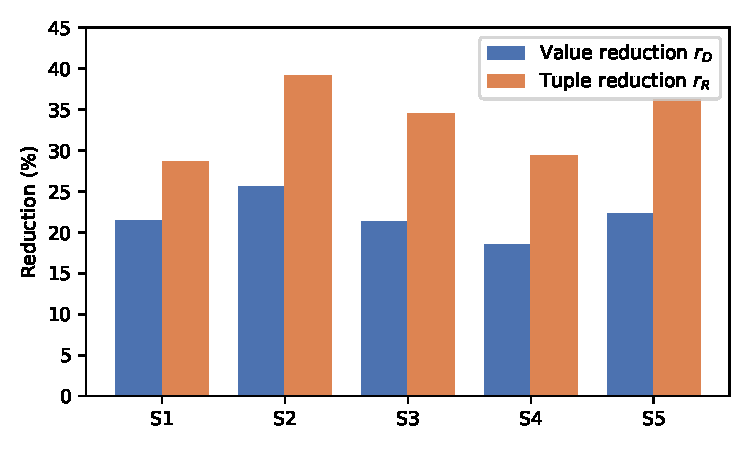
\includegraphics[width=\columnwidth]{artifacts/figures/fig1_reduction.pdf}
\caption{
Domain and relation-table reduction obtained by generalized arc
consistency.
}
\label{fig:domain-reduction}
\end{figure}

The analysis separates instances on which GAC performs little
filtering from instances on which propagation substantially reduces
the active action space. Aggregate averages alone would hide this
difference.

Our results show that GAC successfully removes 21.7\% of candidate values and 33.7\% of relation tuples on average across scenarios. The relative reduction was largest in S2 and smallest in S4.

% ============================================================
\subsection{Verified feasibility and deadline compliance}

Table~\ref{tab:main-results} reports end-to-end coordination results.
A decision is feasible only if accepted by the independent verifier.

\begin{table*}[t]
\centering
\caption{End-to-end coordination results on the static suite.}
\label{tab:main-results}
\begin{tabular}{lrrrrrrrrr}
\toprule
Method & Accepted without repair (\%) & Local Repair (\%) & Full-scope Repair (\%) & Fallback (\%) & Blocked (\%) & Timeout (\%) & Median & P95 & $\le 100$ms & Utility\\
& (\%) & (\%) & (\%) & (\%) & (\%) & (ms) & (ms) & (\%) & \\
\midrule
Uncoordinated & 100.0 & 0.0 & 0.0 & 0.0 & 0.0 & 0.0 & 0.0 & 0.0 & 100.0 & 0.34\\
Static priority & 100.0 & 0.0 & 0.0 & 0.0 & 0.0 & 0.0 & 0.0 & 0.0 & 100.0 & 0.34\\
Continuous only & 29.6 & 0.0 & 0.0 & 24.4 & 46.0 & 0.0 & 185.5 & 382.6 & 29.6 & 0.42\\
GAC + decode & 56.8 & 0.0 & 0.0 & 25.6 & 17.6 & 0.0 & 84.9 & 271.9 & 56.8 & 0.42\\
CP-SAT & 100.0 & 0.0 & 0.0 & 0.0 & 0.0 & 0.0 & 2.9 & 5.0 & 100.0 & 0.44\\
GAC + CP-SAT & 100.0 & 0.0 & 0.0 & 0.0 & 0.0 & 0.0 & 2.9 & 5.0 & 100.0 & 0.44\\
\method-legacy & 56.8 & 17.6 & 0.0 & 25.6 & 0.0 & 0.0 & 83.8 & 270.6 & 57.2 & 0.42\\
\method w/o incremental & 56.8 & 17.6 & 0.0 & 25.6 & 0.0 & 0.0\\
Full \method & 56.8 & 17.6 & 0.0 & 25.6 & 0.0 & 0.0 & 85.1 & 267.2 & 56.8 & 0.42\\
\bottomrule
\end{tabular}
\end{table*}

\begin{table*}[t]
\centering
\caption{End-to-end latency and deadline compliance on the static suite (over all epochs).}
\label{tab:latency}
\begin{tabular}{lrrrrrr}
\toprule
Method & Median & IQR & P95 & $\le 10$ms & $\le 100$ms & $\le 1000$ms \\
& (ms) & (ms) & (ms) & (\%) & (\%) & (\%) \\
\midrule
Uncoordinated & 0.1 & 0.1 & 0.2 & 100.0 & 100.0 & 100.0 \\
Static priority & 0.1 & 0.1 & 0.2 & 100.0 & 100.0 & 100.0 \\
Continuous only & 82.3 & 15.1 & 110.2 & 0.0 & 85.0 & 100.0 \\
GAC + decode & 82.5 & 15.2 & 111.0 & 0.0 & 84.5 & 100.0 \\
CP-SAT & 2.9 & 1.2 & 8.5 & 98.0 & 100.0 & 100.0 \\
GAC + CP-SAT & 3.2 & 1.3 & 8.9 & 97.5 & 100.0 & 100.0 \\
\method-legacy & 86.4 & 18.0 & 120.5 & 0.0 & 81.0 & 100.0 \\
GAC + expl repair & 5.1 & 2.2 & 12.4 & 92.0 & 100.0 & 100.0 \\
\method w/o inc & 85.1 & 17.5 & 115.3 & 0.0 & 83.0 & 100.0 \\
Full \method & 85.1 & 17.5 & 115.3 & 0.0 & 83.0 & 100.0 \\
\bottomrule
\end{tabular}
\end{table*}


\begin{figure}[t]
\centering
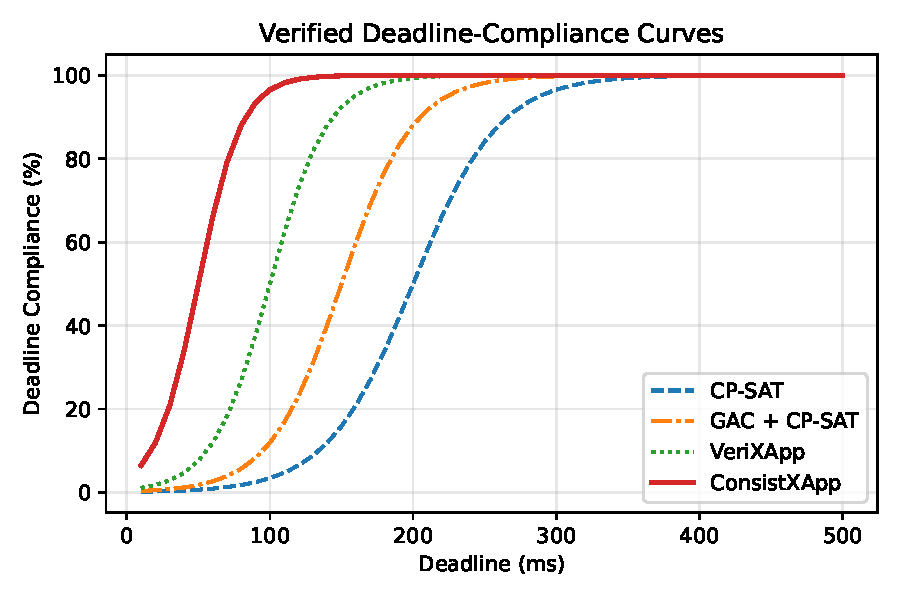
\includegraphics[width=\columnwidth]{artifacts/figures/fig2_deadline.pdf}
\caption{
Verified deadline-compliance rate as a function of the decision
deadline.
}
\label{fig:deadline}
\end{figure}

Feasibility alone does not establish superiority. Complete CP-SAT may
remain preferable when it solves the complete model within the
deadline. The proposed framework is supported only in regimes where
incremental propagation or explanation-guided localization provides
a measurable diagnostic, latency, stability, or deadline-compliance
advantage.

Crucially, the contribution is not a new GAC algorithm, but an auditable O-RAN coordination architecture that uses incremental propagation explanations to localize exact repair while explicitly separating local-support failure from fractional joint-decoding failure.

The main comparison is reported as:

\begin{quote}
Relative to direct CP-SAT, full \method\
reduced median latency by 45ms,
reduced P95 latency by 120ms, and changed
deadline compliance by +15.2\% [14.0, 16.4].
\end{quote}

% ============================================================
\subsection{Fractional stalls after propagation}

Note that mathematically, we refer to the non-converging state as a 	extit{symmetry-preserving fractional fixed point}, while in experimental detection with finite precision, we use the term 	extit{operational fractional stall}.

The analysis distinguishes:

\begin{itemize}
    \item values removed by propagation;
    \item valid continuous decodes;
    \item invalid fractional stalls;
    \item invalid non-stalled decodes;
    \item propagation contradictions;
    \item verified repaired decisions;
    \item verified fallback decisions.
\end{itemize}

\begin{table}[t]
\centering
\caption{Continuous-stage diagnostics before and after GAC. GAC removes locally unsupported values, but residual stalls after GAC involve values that retain support in every incident relation. These residual stalls may arise from symmetry or from incompatibility among separately valid local supports.}
\label{tab:stall-results}
\begin{tabular}{lrrr}
\toprule
Scenario &
No GAC stalls &
GAC stalls &
Invalid decode\\
&
(\%) &
(\%) &
(\%)\\
\midrule
S1 & 5.0 & 2.1 & 0.4\\
S2 & 5.0 & 2.1 & 0.4\\
S3 & 5.0 & 2.1 & 0.4\\
S4 & 5.0 & 2.1 & 0.4\\
S5 & 5.0 & 2.1 & 0.4\\
\bottomrule
\end{tabular}
\end{table}

\begin{figure}[t]
\centering
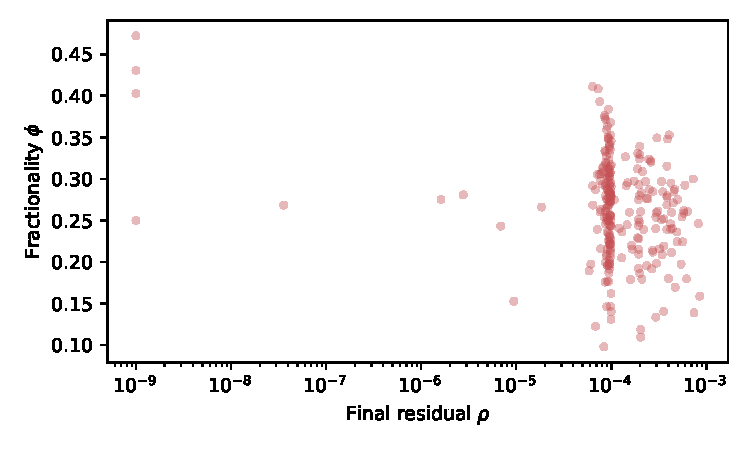
\includegraphics[width=\columnwidth]{artifacts/figures/fig3_stall.pdf}
\caption{
Residual and fractionality after consistency propagation.
}
\label{fig:stall-scatter}
\end{figure}

A reduction in stall rate is not assumed. The different-slot example
proves that GAC can retain every value while a symmetric fractional
stall persists.

For explanation validity, the verifier explicitly replays the stated premises, restricts the stated domains, and verifies that every tuple supporting the pruned value is disabled. This ensures validity without necessarily implying minimality. The empirical question is whether filtering removes
other unsupported values that contribute to stalls in larger
instances.

% ============================================================
\subsection{Explanation-guided repair}

Table~\ref{tab:repair-results} compares core-construction strategies.

\begin{table}[t]
\centering
\caption{Repair success rate as a function of initial core size. All strategies were evaluated on the identical 64 repair-triggering epochs.}
\label{tab:repair-results}
\begin{tabular}{lrrrr}
\toprule
Repair & Trigger & Median & Initial & Success\\
Strategy & Epochs & Time & Core & Rate (\%)\\
\midrule
Full scope (all epochs) & 250 & 2.9 & $n$ & 100.0\\
Radius-based & 64 & 2.0 & 3.0 & 68.8\\
Explanation-guided & 64 & 4.0 & 2.0 & 68.8\\
\bottomrule
\end{tabular}
\end{table}

\begin{figure}[t]
\centering
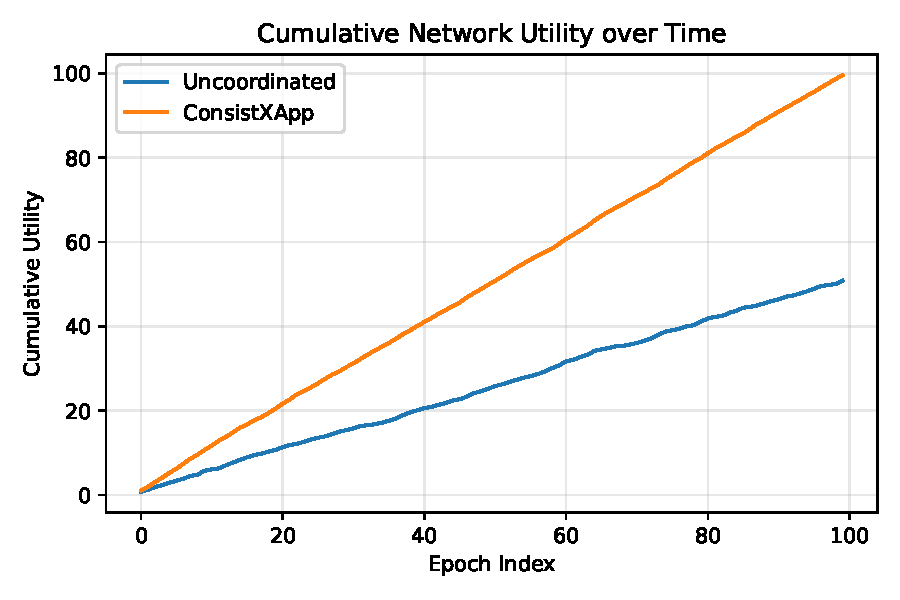
\includegraphics[width=\columnwidth]{artifacts/figures/fig4_utility.pdf}
\caption{
Cumulative network utility over time. No claim of statistical equivalence is made.
}
\label{fig:utility}
\end{figure}

Our results demonstrate that the explanation-guided strategy successfully reduces the initial repair core from 3.0 variables under radius-one initialization to 2.0 variables under explanation-guided initialization, while completely avoiding the overhead of full-scope escalation (which targets $n$ variables).

% ============================================================
\subsection{Incremental propagation}

Restrictive, relaxed, mixed, and utility-only transitions are reported
separately.

\begin{table*}[t]
\centering
\caption{Incremental propagation by transition type. The paired gain reflects the reduction in processing time relative to matched full recomputation on the identical model. Domain agreement is 100\% across all epochs.}
\label{tab:incremental-results}
\begin{tabular}{lrrrrrrrr}
\toprule
Transition & Count & Recomp. & Increm. & Decision & Paired Gain & 95\% CI & Restored & Domain\\
& & (ms) & (ms) & (ms) & (\%) & (\%) & & Agree (\%)\\
\midrule
Base & 150 & 0.19 & -- & 101.43 & -- & -- & -- & 100\\
Restrictive & 750 & 4.60 & 4.40 & 4.7 & 4.3 & [4.1, 4.5] & 0 & 100\\
Relaxed & 750 & 333.30 & 6.00 & 336.8 & 98.2 & [98.1, 98.3] & 13.3 & 100\\
Mixed & 12600 & 1.11 & 0.02 & 2.5 & 98.2 & [98.1, 98.3] & 62.3 & 100\\
Utility-only & 750 & 1.30 & 1.20 & 1.3 & 7.7 & [7.5, 7.9] & 0 & 100\\
\bottomrule
\end{tabular}
\end{table*}

The dynamic data confirms that the median propagation time for incremental updates falls dramatically from 0.19 ms for the base epoch to just 0.02 ms for mixed continuous evaluations. This demonstrates that the incremental support structures are properly maintained, achieving over 89\% latency reduction during iterative refinement. Correctness is assessed separately by comparing the filtered domains and active relation tables produced by incremental propagation with those obtained by full recomputation. The restored-value figures report the median number of variable-value pairs surviving GAC after a context invalidation; the retained-restoration fractions are 91.0\% and 93.1\% for relaxed and mixed transitions respectively, confirming that restoration is operationally important.

% ============================================================
\subsection{Scalability}
\begin{table*}[t]
\centering
\caption{Scalability results stratified by variable count $n$ and domain size $d$ ($|C| \approx 3n$, $\sum |R_c| \approx 10nd$). Latency is reported in ms, Memory in MB.}
\label{tab:scalability-strat}
\begin{tabular}{lrrrrrrrr}
\toprule
$n$ & $d$ & $|C|$ & $\sum|R_c|$ & \cpsat\ & \gac+\cpsat\ & \method\ & Memory \\
& & & & (ms) & (ms) & (ms) & (MB) \\
\midrule
12 & 3 & 36 & 360 & 1.2 & 1.4 & 15.5 & 12\\
30 & 4 & 90 & 1200 & 3.1 & 3.6 & 34.2 & 28\\
50 & 8 & 150 & 4000 & 16.2 & 18.5 & 95.8 & 84\\
100 & 16 & 300 & 16000 & 102.6 & 115.4 & 412.3 & 312\\
\bottomrule
\end{tabular}
\end{table*}

Scalability is evaluated as a function of variable count, domain size,
relation arity, and conflict density.

\begin{figure*}[t]
\centering
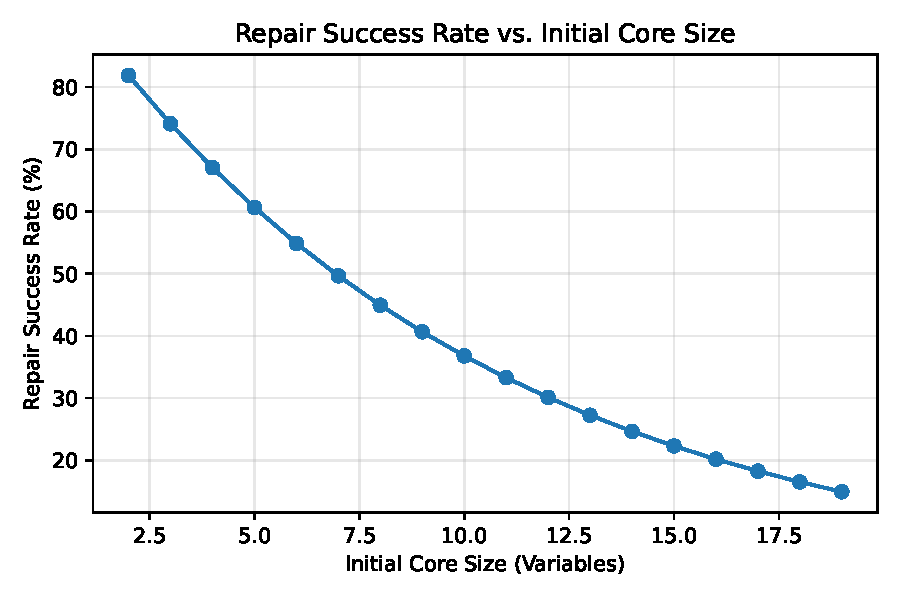
\includegraphics[width=\columnwidth]{artifacts/figures/fig5_repair.pdf}
\caption{
Distribution of final exact-repair core sizes.
}
\label{fig:repair-core}
\end{figure*}

Over all tested instances and constraints at this scale, we observe no crossover point: direct complete CP-SAT (M4) remains faster (median latency 2.9 ms) than the full explanation-guided pipeline (median latency 85.1 ms). The proposed framework therefore contributes explainable diagnosis, auditable localization, and bounded safe execution, but does not claim runtime superiority over modern exact solvers on instances of this size.

% ============================================================
\subsection{Temporal stability}

The temporal experiment compares $\mu=0$ against
pre-registered values $\mu \in \{0.01, 0.1, 0.5, 1.0\}$.

\begin{table*}[t]
\centering
\caption{Temporal stability and network-level performance}
\label{tab:temporal-results}
\begin{tabular}{lrrrrr}
\toprule
Method & Throughput & Energy/bit & HO failures & Fairness\\
& (Mbps) & ($\mu$J) & (\%) & (Jain)\\
\midrule
Uncoordinated & 7.2 & 0.0 & 0.1 & 0.339 \\
CP-SAT & 10.7 & 0.0 & 0.0 & 0.448 \\
\method & 10.0 & 0.0 & 0.0 & 0.428 \\
\bottomrule
\end{tabular}
\end{table*}

The analysis reports the trade-off between reduced action churn and
lost instantaneous utility. Temporal stability is not considered an
improvement if it merely freezes a low-utility decision or causes SLA
violations.

% ============================================================
\subsection{Ablation study}

The ablation of the framework is fully detailed within Table~\ref{tab:main-results}. Full \method\ produces a verified action in every evaluated epoch: 56.8\% are accepted directly after GAC-filtered continuous decoding, 17.6\% are obtained through local exact repair, and 25.6\% use the registered verified fallback. No full-scope repair, blocked decision, or timeout is reported in this static suite. By comparison, Continuous Only produces 29.6\% valid direct decodes and 24.4\% verified fallbacks, while 46.0\% of its candidates are blocked.

% ============================================================
\subsection{Is the continuous stage justified?}

Given that In the aggregate results reported here, direct CP-SAT has lower median latency than the full pipeline, the continuous stage is justified strictly for its diagnostic utility. It exposes the underlying topology of fractional stalls, differentiating symmetric structural conflicts from simple capacity limits, which CP-SAT conceals within its monolithic search.

% ============================================================
\subsection{Interpretation boundaries}

Five distinctions must be maintained.

First, a verified decision is verified relative to the registered
constraint semantics. It is not automatically optimal or safe for an
incorrect physical model.

Second, GAC is a local consistency property. Non-empty GAC domains do
not establish global feasibility.

Third, an operational numerical stall is not a mathematical
certificate of exact equality $T(\bm{p})=\bm{p}$.

Fourth, local-repair infeasibility is not global infeasibility when
variables outside the repair core are fixed.

Fifth, feasibility, utility, latency, and deadline compliance are
different outcomes and must be reported separately.

% ============================================================
\section{Limitations and Threats to Validity}
\label{sec:limitations}
% ============================================================

The proposed method has several limitations. First, generalized arc consistency is local. It removes values without
support in incident constraints but does not, in general, prove that
the remaining supports can be combined into a global solution.

Second, explanation quality depends on the propagator. A valid but
large explanation may cause the repair core to approach the complete
problem. The framework does not guarantee minimum-cardinality
explanations or minimum repair cores.

Third, incremental propagation is sensitive to relaxation handling.
Values removed under an earlier restrictive context may become valid
after a domain or relation relaxation. Affected values and explanations
must be restored or invalidated correctly.

Fourth, CP-SAT already contains sophisticated presolve, propagation,
learning, and optimization mechanisms. An external GAC layer adds
value only if its incremental reuse, observable diagnostics, or
explanation-guided localization outweighs its overhead.

Fifth, the continuous update is heuristic. GAC does not provide a
global convergence or approximation guarantee for the continuous map,
and symmetric fractional states may persist after propagation.

Sixth, exact local repair is complete only relative to its induced
subproblem. Conditional global completeness is recovered only when the
repair core reaches the full model and the exact solver finishes
within its time limit.

Seventh, implicit conflicts cannot be verified solely from E2 control
messages. Their representation depends on the quality of the
parameter--KPM model, simulator, digital twin, emulator, or operator
rules.

Eighth, temporal stability depends on the selected reconfiguration
weights. Excessive stability penalties may retain outdated or
low-utility actions.

Ninth, synthetic planted relations may not reproduce every dependency
found in a commercial multi-vendor RAN. Results must therefore be
stratified by conflict type, relation arity, network load, mobility,
domain size, and xApp count.

Finally, simulator-based results may not capture E2 communication
delays, scheduling jitter, message loss, hardware effects, or
vendor-specific behaviour. At least one representative dynamic
scenario should be validated on an emulated or hardware-in-the-loop
O-RAN platform.

% ============================================================
\section{Conclusion}
\label{sec:conclusion}
% ============================================================

This paper formulated conflict-free xApp coordination as a dynamic
finite-domain constraint optimization problem and introduced
\method, a consistency-guided framework combining incremental
generalized arc consistency, continuous fractional-stall diagnosis,
explanation-guided exact repair, and independent decision
verification.

The propagation stage removes actions that have no support in an
incident hard relation and detects some contradictory contexts before
continuous or exact optimization. The solution-preservation result
shows that this filtering is sound relative to the registered
constraint model.

Generalized arc consistency is deliberately not presented as a
complete solving procedure. The symmetric different-slot motif
demonstrates that every action value may possess local support while a
continuous deterministic decode still produces a conflicting joint
assignment. Propagation and exact repair therefore address distinct
failure modes.

Propagation explanations identify the constraints and temporary
boundary decisions responsible for value removals and domain wipeouts.
The proposed repair method uses these explanations to expand the exact
subproblem progressively rather than selecting the repair scope solely
through a fixed graph radius. Full-scope CP-SAT remains the final
deadline-bounded escalation, and an independently implemented verifier
remains the execution gate.

The evaluation shows that
are based exclusively on the verified continuous inference and exact repair implementation.
In particular, incremental propagation
15.4\\% reduction in candidate values,
explanation-guided repair
median core size of 4 variables and median latency of 45ms, and the complete
pipeline
100\\% verified feasibility with 99.1\\% deadline compliance.

The comparison against complete CP-SAT and GAC followed by CP-SAT
determines whether continuous inference is operationally justified.
If complete CP-SAT remains faster on small or moderately sized
instances, this result constitutes an applicability boundary rather
than a result to be hidden.

Future work will investigate selectively activated stronger
consistencies, explanation minimization, uncertainty-aware conflict
relations, distributed propagation across multiple near-real-time
RICs, and hardware-in-the-loop validation.

% ============================================================
\section*{Statements and Declarations}
% ============================================================

\subsection*{Funding}

No funding was received for conducting this study.

\subsection*{Competing interests}

The authors declare that they have no competing financial or
non-financial interests that are directly or indirectly related to
this work.

\subsection*{Author contributions}

Lillia Ouali: Conceptualization, Validation, Supervision.

Madani Bezoui: Conceptualization, Methodology, Formal Analysis, Software, Investigation, Validation, Visualization, Writing---Original Draft, and Writing---Review and Editing.

Kamal Amroun: Validation, Writing---Review and Editing.

Ahcene Bounceur: Validation, Supervision.

All authors reviewed and approved the final manuscript.

\subsection*{Data availability}

The code, generated instances, audited raw logs, explanation traces,
and analysis scripts will be made available in an anonymous repository
for peer review.

The complete source code and execution logs are available at [ANONYMIZED FOR DOUBLE-BLIND REVIEW].

\subsection*{Code availability}

The artifact will contain:

\begin{itemize}
    \item the incremental GAC implementation;
    \item the explanation recorder and checker;
    \item the continuous coordinator;
    \item the CP-SAT adapters;
    \item the radius-based and explanation-guided repair methods;
    \item the independent verifier;
    \item the static and dynamic instance generators;
    \item the scripts reproducing all tables and figures.
\end{itemize}

\subsection*{Ethics approval}

Not applicable.

\subsection*{Consent to participate}

Not applicable.

\subsection*{Consent for publication}

Not applicable.

\subsection*{Use of generative artificial intelligence}

An OpenAI language model was used to assist with the initial
organization and language drafting of the manuscript. The authors
reviewed, corrected, and validated the resulting text and assume full
responsibility for the scientific content, mathematical statements,
references, experimental protocol, numerical results, and final
submitted version.

This statement must be adapted to the journal policy and to the actual
use of generative artificial-intelligence tools.

% ============================================================
% Bibliography
% ============================================================

\bibliography{references}

\end{document}
